%
%   Copyright 2013 Katarzyna Szawan <kat.szwn@gmail.com>
%       and Michał Rus <m@michalrus.com>
%
%   Licensed under the Apache License, Version 2.0 (the "License");
%   you may not use this file except in compliance with the License.
%   You may obtain a copy of the License at
%
%       http://www.apache.org/licenses/LICENSE-2.0
%
%   Unless required by applicable law or agreed to in writing, software
%   distributed under the License is distributed on an "AS IS" BASIS,
%   WITHOUT WARRANTIES OR CONDITIONS OF ANY KIND, either express or implied.
%   See the License for the specific language governing permissions and
%   limitations under the License.
%

\subsection{User interface mock-ups}
\label{subsec:ui-mockups}

\Cref{fig:mockup-maplist} below show a \emph{mock-up} (a sketch) of the main, initial screen of the Android application. The user can:

\begin{itemize}
	\item choose an existing map to edit,
	\item select and delete a map by long-pressing it,
	\item add a new map,
	\item import an existing XMind map,
	\item switch to any other opened map by means of tabs at the top.
\end{itemize}

\begin{figure}[h]
	\centering
	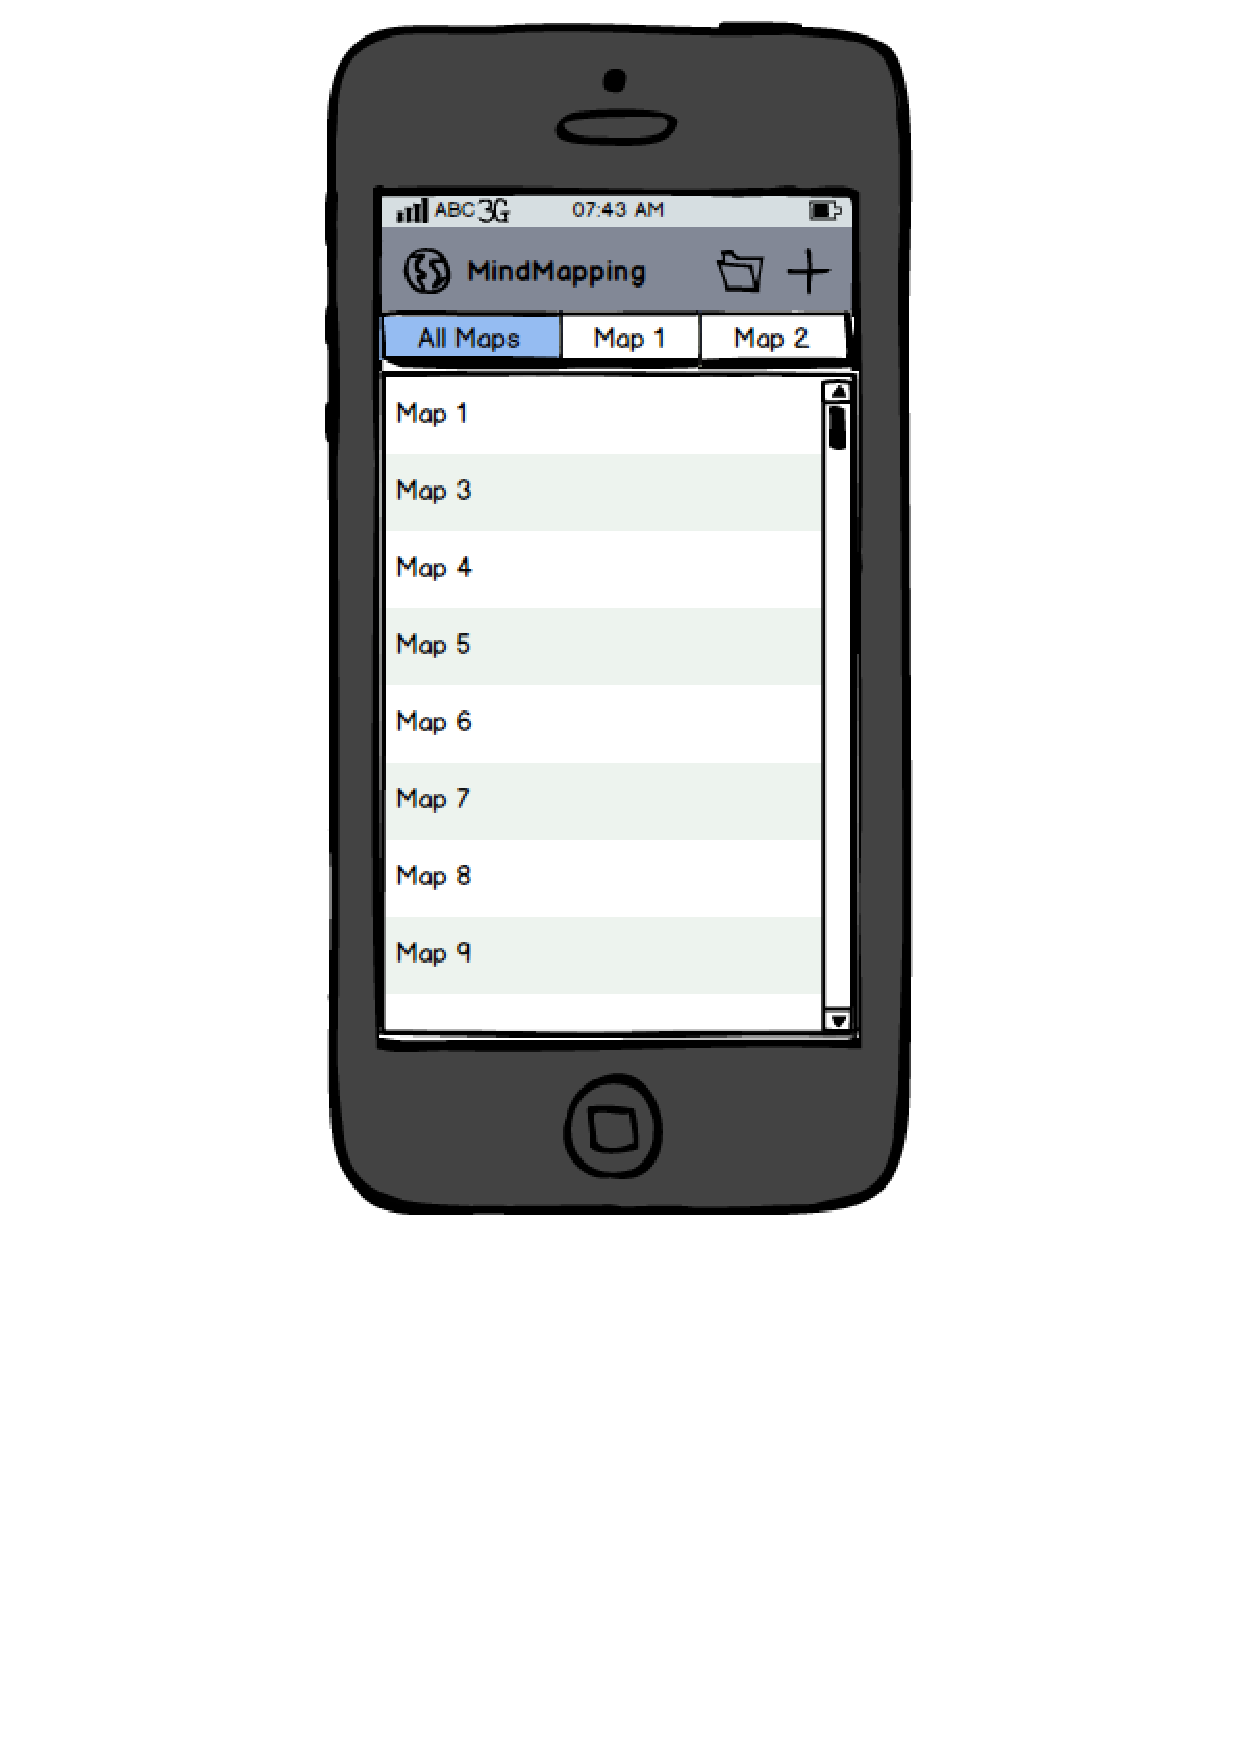
\includegraphics[width=0.5\textwidth]{graphics-mockup-list}
	\caption{Mock-up of mind map list, initial screen.}
	\label{fig:mockup-maplist}
\end{figure}

\Cref{fig:mockup-mindmap} shows a similar preview of a map view: a screen that is shown to the user when he chooses/adds/imports a map in \cref{fig:mockup-maplist}. Here, the user can:

\begin{itemize}
	\item edit content of any `mind node' by tapping on it,
	\item remove any node (and its subtree) by long-pressing it and selecting `remove',
	\item move any node (reassign its parent node) by long-pressing it and selecting `change parent', and then tapping on the new parent,
	\item add a child node to any node by tapping on `+' button next to the parent node,
	\item see (in real-time) changes introduced by other editors currently editing this map.
\end{itemize}

\begin{figure}[h]
	\centering
	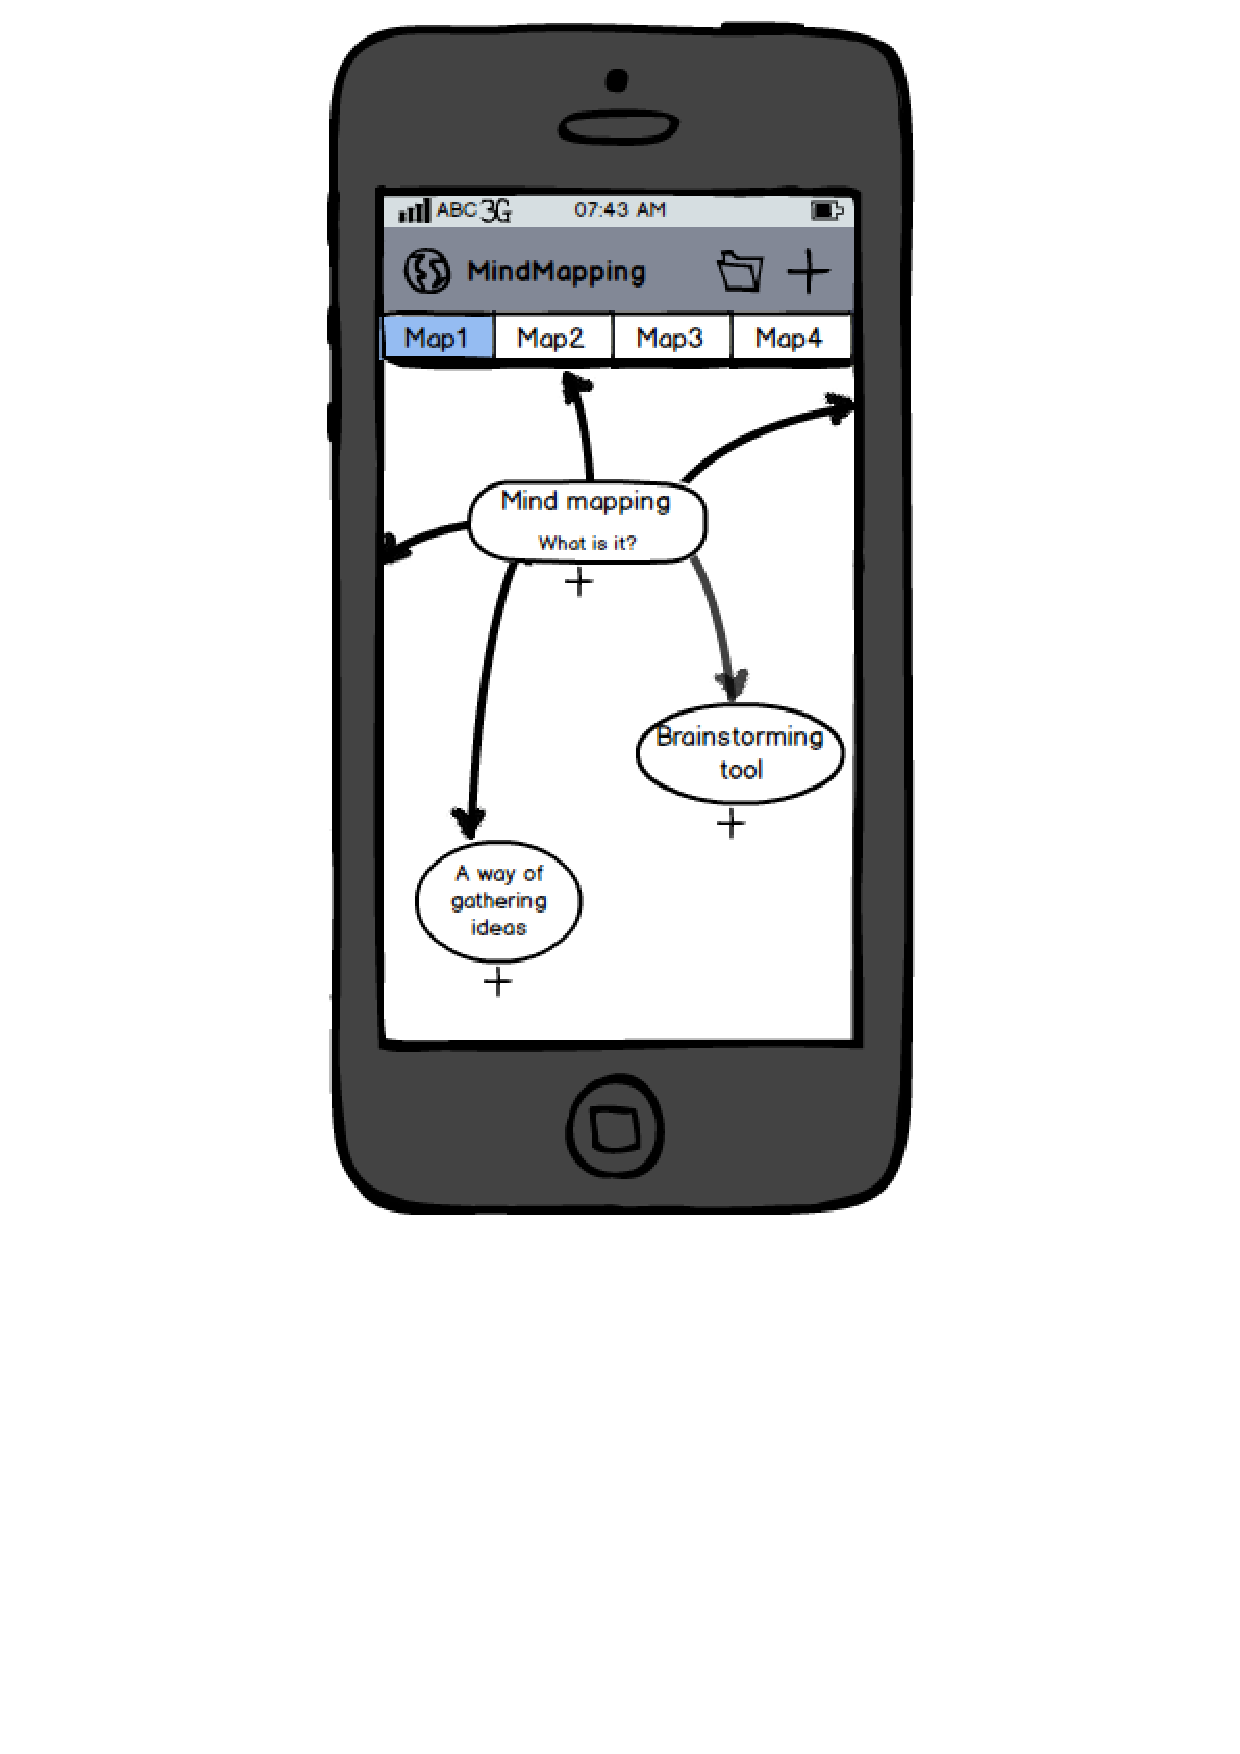
\includegraphics[width=0.5\textwidth]{graphics-mockup-map}
	\caption{Mock-up of mind map view.}
	\label{fig:mockup-mindmap}
\end{figure}

\todo[inline,caption=\michal{K., any more mock-ups needed?}
\kasia{I think it's enough. Now we need to fit the size of the images}]{}
